%==============================================================

\chapter{Big Data Framework Spark}\label{bds1}

After accumulating the Data and presenting various methods to extract different audio features, the following chapters describe the data analysis with Apache Spark \cite{spark}. Chapter \ref{bds1} deals with the implementation of the various similarity measurements while chapter \ref{bds2} deals with the handling of larger amounts of data, runtime analysis and the combination of multiple similarity measurements. 

\section{Apache Hadoop and Spark} 

First of all a small introduction to Big Data processing with Spark is given.
With the ever growing availability of huge amounts of high dimensional data the need for toolkits and efficient algorithms to handle these grew as well over the past years. Map-Reduce as a 

\subsection{Hadoop and Map Reduce}

\subsection{Spark and RDDs}

\subsection{Spark DataFrame}

\subsection{lazy evaluation}

\subsection{Performance Comparison of RDD vs DataFrame}


\textit{insert plot here}
\begin{figure}[htbp]
	\centering
	\framebox{\parbox{1\textwidth}{
			\begin{subfigure}{.495\textwidth}
				\centering
				\includegraphics[scale=0.22]{Images/Spark/spark_cluster_rdd_1517.png}
				\caption{RDD on Cluster, 3180 songs}
				\label{sc1}
			\end{subfigure}%
			
			\begin{subfigure}{.495\textwidth}
				\centering
				\includegraphics[scale=0.22]{Images/Spark/df_vs_dfmerged_full.png}
				\caption{DataFrame on single Node}
				\label{sc2}
			\end{subfigure}% 			
	}}
	\caption{Spark RDD vs Dataframe}
	\label{fig:spark1}
\end{figure}

\subsection{min and max value aggregation}

\section{Data aggregation}

To work with the features a few transformations have to be done first. 

\begin{pythonCode}
song = "music/TURCA1.wav"
chroma = sc.textFile("features/out[0-9]*.notes")
chroma = chroma.map(lambda x: x.split(';'))
chroma = chroma.map(lambda x: (x[0], x[1], x[2], x[3].replace("10",'K').replace("11",'L').replace("0",'A').replace("1",'B').replace("2",'C').replace("3",'D').replace("4",'E').replace("5",'F').replace("6",'G').replace("7",'H').replace("8",'I').replace("9",'J')))
chroma = chroma.map(lambda x: (x[0], x[1], x[2], x[3].replace(',','').replace(' ','')))
df = spark.createDataFrame(chroma, ["id", "key", "scale", "notes"])
\end{pythonCode}

\section{Euclidean Distance}

\begin{pythonCode}
distance_udf = F.udf(lambda x: float(distance.euclidean(x, comparator_value)), FloatType())
result = df_vec.withColumn('distances', distance_udf(F.col('features')))
result = result.select("id", "distances").orderBy('distances', ascending=True)
result = result.rdd.flatMap(list).collect()
\end{pythonCode}

\section{Bucketed Random Projection}

\begin{pythonCode}
brp = BucketedRandomProjectionLSH(inputCol="features", outputCol="hashes", seed=12345, bucketLength=1.0)
model = brp.fit(df_vec)
comparator_value = Vectors.dense(comparator[0])
result = model.approxNearestNeighbors(df_vec, comparator_value, df_vec.count()).collect()
rf = spark.createDataFrame(result)
result = rf.select("id", "distCol").rdd.flatMap(list).collect()
\end{pythonCode}


\section{Cross-correlation}

\textit{\textbf{2 Versions explained - with additional key shift and without}}

\begin{pythonCode}
def chroma_cross_correlate(chroma1, chroma2):
    corr = sc.signal.correlate2d(chroma1, chroma2, mode='full') 
    transposed_chroma = np.transpose(corr)
    mean_line = transposed_chroma[12]
    return np.max(mean_line)
distance_udf = F.udf(lambda x: float(chroma_cross_correlate(x, comparator_value)), DoubleType())
result = df_vec.withColumn('distances', distance_udf(F.col('chroma')))
result = result.select("id", "distances").orderBy('distances', ascending=False)
result = result.rdd.flatMap(list).collect()
\end{pythonCode}


\textbf{Memory intense - had to alter spark-defaults.conf}
\textit{spark.driver.memory             6g\\
spark.executor.memory           2g\\
}


\section{Kullback-Leibler Divergence}

\begin{pythonCode}
def symmetric_kullback_leibler(vec1, vec2):
	#preprocessing: splitting vec1 and vec2 into mean1, mean2, cov1 and cov2
    d = 13
    div = 0.25 * (np.trace(cov1 * np.linalg.inv(cov2)) + np.trace(cov2 * np.linalg.inv(cov1)) + np.trace( (np.linalg.inv(cov1) + np.linalg.inv(cov2)) * (mean1 - mean2)**2) - 2*d)
    return div
distance_udf = F.udf(lambda x: float(symmetric_kullback_leibler(x, comparator_value)), DoubleType())
result = df_vec.withColumn('distances', distance_udf(F.col('features')))
result = result.select("id", "distances").orderBy('distances', ascending=True)
result = result.rdd.flatMap(list).collect()
\end{pythonCode}


\section{Jensen-Shannon Divergence}

\begin{pythonCode}
def jensen_shannon(vec1, vec2):
	#preprocessing: splitting vec1 and vec2 into mean1, mean2, cov1 and cov2
    mean_m = 0.5 * (mean1 + mean2)
    cov_m = 0.5 * (cov1 + mean1 * np.transpose(mean1)) + 0.5 * (cov2 + mean2 * np.transpose(mean2)) - (mean_m * np.transpose(mean_m))
    div = 0.5 * np.log(np.linalg.det(cov_m)) - 0.25 * np.log(np.linalg.det(cov1)) - 0.25 * np.log(np.linalg.det(cov2))  
    if np.isnan(div):
        div = np.inf
    return div
distance_udf = F.udf(lambda x: float(jensen_shannon(x, comparator_value)), DoubleType())
result = df_vec.withColumn('distances', distance_udf(F.col('features')))
result = result.select("id", "distances").orderBy('distances', ascending=True)
result = result.rdd.flatMap(list).collect()

\end{pythonCode}

\textit{Problem mit den "skyrocketing determinanten" -> Lösung: cholesky zerlegung, geht nicht - nicht positiv definit}\cite[p.45]{schnitzer1}

\section{Levenshtein distance}

\begin{pythonCode}
def get_neighbors_notes(song):
    filterDF = df.filter(df.id == song)
    filterDF.first()
    comparator_value = filterDF.collect()[0][3] 
    print comparator_value
    df_merged = df.withColumn("compare", lit(comparator_value))
    df_levenshtein = df_merged.withColumn("word1_word2_levenshtein", levenshtein(col("notes"), col("compare")))
    df_levenshtein.sort(col("word1_word2_levenshtein").asc()).show()
\end{pythonCode}

\section{Andere MapReduce tasks}

\subsection{Alternating Least Squares}

\subsection{TF-IDF weights}

\subsection{DIMSUM all-pairs similarity}

\section{Combining different measurements}

\textit{\textbf{Pre- merge feature sets, broadcast comparator, descending importance pre-filtering}}

\textit{\textbf{statistic normalization of similarities}}

\section{performance}


\begin{figure}[htbp]
	\centering
	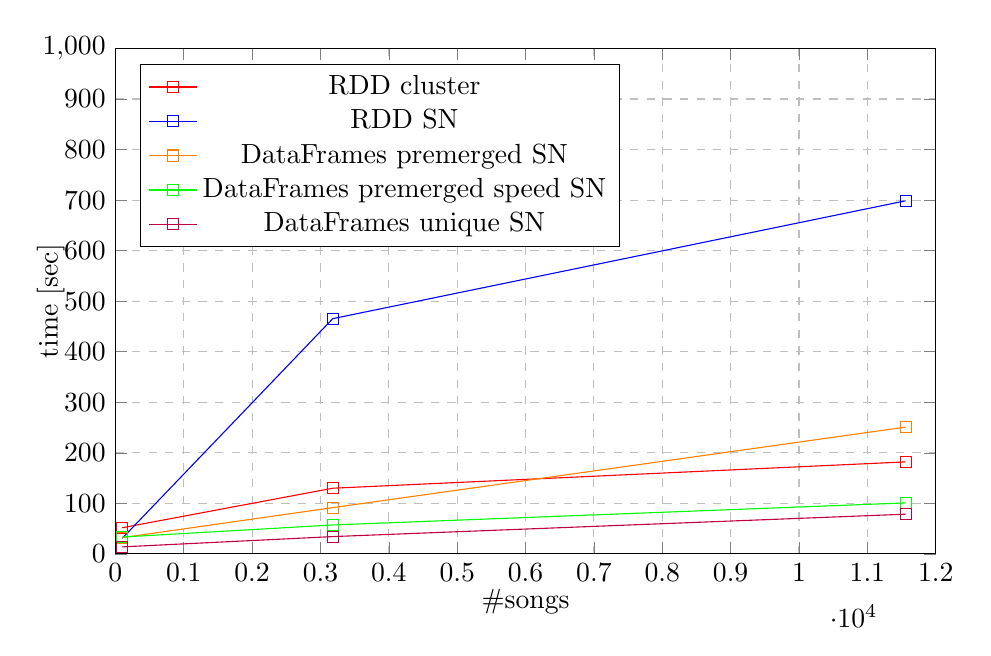
\begin{tikzpicture}
	\centering
	\begin{axis}[
	    %title={Performance of various toolkits},
		x label style={at={(axis description cs:0.5,-0.05)},anchor=north},
		y label style={at={(axis description cs:-0.05,.5)},rotate=0,anchor=south},
	    xlabel={\#songs},
	    ylabel={time [sec]},
	    xmin=0, xmax=12000,
	    ymin=0, ymax=1000,
	    xtick={0,1000,2000,3000,4000,5000,6000,7000,8000,9000,10000,11000,12000},
	    ytick={0,100,200,300,400,500,600,700,800,900,1000},
	    legend pos=north west,
	    ymajorgrids=true,
	    grid style=dashed,
	    height=8cm,
	    width=12cm,
	    grid=major,
	]
	\addplot[
		color=red,
		mark=square,
		]
		coordinates {
	    (100,51.736)(3180,129.940)(11560,182.035)
		};
		\addlegendentry{RDD cluster}
	\addplot[
	    color=blue,
	    mark=square,
	    ]
	    coordinates {
	    (100,30.770)(3180,465.445)(11560,698.657)
	    };
	    \addlegendentry{RDD SN}
	\addplot[
	    color=orange,
	    mark=square,
	    ]
	    coordinates {
	    (100,32.087)(3180,91.477)(11560,250.854)
	    };
	    \addlegendentry{DataFrames premerged SN}
	  
	\addplot[
	    color=green,
	    mark=square,
	    ]
	    coordinates {
	    (100,33.351)(3180,57.230)(11560,100.884)
	    };
	    \addlegendentry{DataFrames premerged speed SN}

	\addplot[
	    color=purple,
	    mark=square,
	    ]
	    coordinates {
	    (100,13.874)(3180,34.232)(11560,78.566)
	    };
	    \addlegendentry{DataFrames unique SN}	    
	\end{axis}
	\end{tikzpicture}
	\caption{Performance of various spark algorithms}
	\label{perfspark}
\end{figure}

\textit{\textbf{high data locality, full parallelizable, very low replication rate}}

\textit{\textbf{insert data locality scheme here}}

Very small 100 Song Dataset plus 20 Cover Songs to evaluate and compare similarity metrics. Full similarity matrices. 
High performance/ throughput tests with full 12000 song testset to evaluate full load performance.\\


\section{feature separation quality}